\documentclass[aspectratio=1610,compress,t,gabaritb,french,english]{hecppt}

%% Packages
\usepackage{fontawesome}
\usepackage{metalogo}
\usepackage{listings}
\usepackage{tabularx}
\usepackage{colortbl}
\usepackage{hyperref}

%% Commandes
\newcommand{\cmd}[1]{%
	\texttt{\textbackslash #1}
}

%% Environnements
\lstnewenvironment{codesource}{%
	\lstset{%
		basicstyle=\tiny,
		language=[LaTeX]TeX,
		backgroundcolor=\color{bleuPaleSecondaire!10},
		tabsize=2,
		% frame=leftline,
		% numbers=left,
		% numberstyle=\tiny,
		literate=%
		{à}{{\`a}}1
		{é}{{\'e}}1
		{ç}{{\c c}}1
		{«}{{\og}}1
		{»}{{\fg}}1
	}
}{}

%% Options des packages
\hypersetup{colorlinks=true,%
	urlcolor=bleuFoncePrimaire,%
	linkcolor=bleuFoncePrimaire,%
	pdfauthor=Benoit Hamel,%
	pdftitle=Rédaction avec LaTeX : Principes de base}
\frenchbsetup{og=«,fg=»}
\setlength{\parskip}{1ex}

%% Métadonnées du document

\title{Writing with \\ \texttt{\textbackslash title}\{\textrm{\LaTeX}\} }
\subtitle{The Basics}
\HECauteur{Benoit Hamel}{Benoit Hamel}
\date[2018-02-28]{2018-02-28}
\subject{} % Sujet inséré dans les métadonnées du pdf
\keywords{} % Mots-clés insérés dans les métadonnées du pdf

\begin{document}

\pageTitre

% Pages liminaires
\scriptsize

% Page titre
\begin{frame}
	Benoit Hamel \\
	Technicien en documentation, soutien technique \\
	Bibliothèque HEC Montréal
	\vfill
	{
		\Huge\bfseries
		Rédaction avec \\
		\texttt{\textbackslash title\{\textrm{\LaTeX}\}}
	}
	\vfill
	Première partie : Principes de base \\
	Édition HEC Montréal, revue et augmentée (version française)
\end{frame}

% Page de la licence
\begin{frame}
	\faCopyright\ 2016 Vincent Goulet pour la 
	\href{https://ctan.org/pkg/formation-latex-ul}{version originale}. La liste des sources qui ont 
	servi à l'élaboration de cette formation se trouve à la fin du présent document.
	
	\faCreativeCommons\ Cette création est mise à disposition selon le contrat 
	\href{http://creativecommons.org/licenses/by-sa/4.0/deed.fr}{%
	Attribution-Partage dans les mêmes conditions 4.0 International de Creative Commons}. 
	En vertu de ce contrat, vous êtes libre de :
	
	\begin{itemize}
		\item partager -- reproduire, distribuer et communiquer l’oeuvre;
		\item remixer -- adapter l’oeuvre;
		\item utiliser cette oeuvre à des fins commerciales.
	\end{itemize}

	Selon les conditions suivantes :
	
	\begin{itemize}
		\item Attribution -- Vous devez créditer l’oeuvre, intégrer un lien vers le contrat et indiquer si des modifications ont été effectuées à l’oeuvre. Vous devez indiquer ces informations par tous les moyens possibles, mais vous ne pouvez suggérer que l’Offrant vous soutient ou soutient la façon dont vous avez utilisé son oeuvre.
		\item Partage dans les mêmes conditions -- Dans le cas où vous modifiez, transformez ou créez à partir du matériel composant l’oeuvre
		originale, vous devez diffuser l’oeuvre modifiée dans les même conditions, c’est-à-dire avec le même contrat avec lequel l’oeuvre originale a été diffusée.
	\end{itemize}
\end{frame}

% Table des matières
\begin{frame}{Sommaire de la formation}
	\begin{columns}[onlytextwidth]
		\begin{column}{.49\textwidth}
			\tableofcontents[sections={1-3}]
		\end{column}
		\begin{column}{.49\textwidth}
			\tableofcontents[sections={4-6}]
		\end{column}
	\end{columns}
\end{frame}
% Présentation de TeX et LaTeX
\small

\section{\TeX\ and \LaTeX\ presentation}

\subsection{What is \TeX\ and \LaTeX?}

\begin{frame}[c,label=fr:commencement]{At the beginning (1978), there was \TeX\ldots}
	
\includegraphics[width=\textwidth,keepaspectratio=true]{knuth-tex-commencement.jpg}
\end{frame}

\begin{frame}[c]{What is \TeX?}

	\begin{itemize}
		\item A typesetting and document preparation system;
		\item ``The most powerful formatting program for producing book-quality text 
			of scientific and technical works''\footnote{Kopka \& Daly, p. 6};
		\item A mature, stable, complete and bug-free system;
		\item A set of very primitive commands perfect for typography and
			programming functions;
		\item «\emph{typesetter-level program}».
	\end{itemize}

\end{frame}

\begin{frame}[c,label=fr:sixiemejour]{On the sixth day (1983), there was \LaTeX\ldots}
	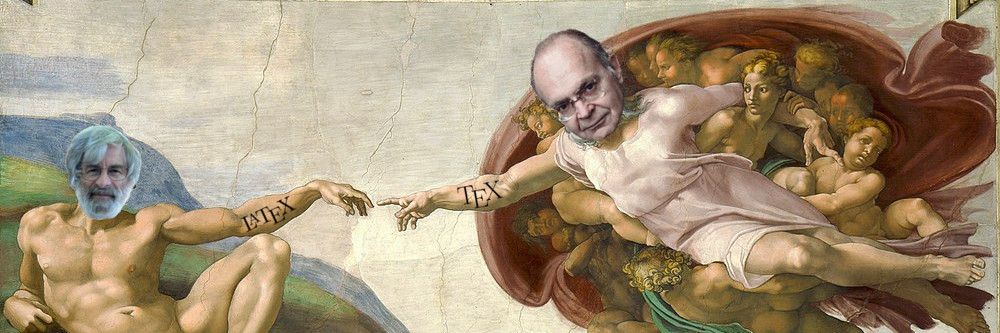
\includegraphics[width=\textwidth,keepaspectratio=true]{creation-of-latex.jpg}
\end{frame}

\begin{frame}{What is \LaTeX?}
	\begin{itemize}
		\item A set of macro-commands used to facilitate \TeX's usage;
		\item No preliminary knowledge of typography in general or \TeX\ in particular
			is required;
		\item Typographical and logical markup language used for text layout (like HTML);
		\item Cross-platform language, identical from one operating system to the other,
			and extensible with packages;
		\item «\emph{author-level program}».
	\end{itemize}
\end{frame}

\subsection{A \LaTeX\ document creation process}

% Rédiger avec une nouvelle perspective
\begin{frame}[c]{Writing with a new perspective}
	
	\begin{itemize}
		\item You write your document in plain text and use commands to describe
			\textbf{what your text is} and \textbf{not what it's supposed to look like}.
		\item You concentrate on your \textbf{content}.
		\item You let \LaTeX\ do its work, that is taking care of the \textbf{container}.
	\end{itemize}
	
\end{frame}

% Processus de création d'un document LaTeX
\begin{frame}[c]{\LaTeX\ document creation process}
	\Huge
	\begin{minipage}[t]{0.25\linewidth}
		\centering
		\faFileTextO
	\end{minipage}
	\hfill\faArrowRight\hfill
	\begin{minipage}[t]{0.25\linewidth}
		\centering
		\faCogs
	\end{minipage}
	\hfill\faArrowRight\hfill
	\begin{minipage}[t]{0.25\linewidth}
		\centering
		\faFilePdfO
	\end{minipage}

	\begin{picture}(0,0)
		\footnotesize\thicklines\color{bleuFonceSecondaire}
		\onslide<2>\put(0,-10){\dashbox{1}(35,40)[b]{\parbox{.2\textwidth}{\centering\textbf{text writing and markup in a text editor\smallskip}}}}
		\onslide<3>\put(54,-10){\dashbox{1}(35,40)[b]{\parbox{.2\textwidth}{\centering\textbf{compilation with a \TeX\ engine from the command line\smallskip}}}}
		\onslide<4>\put(108,-10){\dashbox{1}(35,40)[b]{\parbox{.2\textwidth}{\centering\textbf{visualization with an external viewer\smallskip}}}}
	\end{picture}
\end{frame}
% Principes de base

\section{The Basics}

\subsection{Document Structure}

% Structure d'un document
\begin{frame}[fragile]{Document structure}

	Un document \LaTeX\ est toujours composé de deux parties :
	
\begin{codesource}
	
	\documentclass[11pt,french]{article}
	\usepackage[utf8]{inputenc}
	\usepackage[T1]{fontenc}
	\usepackage{babel}
	\usepackage[autolanguage]{numprint}
	
	\begin{document}
		
		\section{Primo}
		
		Ac class dis donec erat facilisis magna mattis 
		placerat potenti praesent primis sed tellus turpis 
		ut vehicula. Ad amet eleifend eros fames habitant 
		imperdiet integer laoreet leo magna magnis neque 
		netus senectus taciti torquent. 
		
		\section{Deuxio}
		
		Cursus dui egestas eget eros et hac magna massa mollis 
		natoque penatibus sagittis sed tellus urna velit 
		vestibulum vitae vulputate. 
	\end{document}
\end{codesource}

	\begin{picture}(0,0)
		\thicklines\color{bleuFonceSecondaire}
		\onslide<2>\put(1,47){\dashbox{1}(87,15){}}
		\onslide<2>\put(89,53){\Large\textbf{\faArrowLeft\ Préambule}}
		\onslide<3>\put(1,6){\dashbox{1}(87,41){}}
		\onslide<3>\put(89,24){\Large\textbf{\faArrowLeft\ Corps du document}}
	\end{picture}
\end{frame}

% Préambule : la classe de document
\begin{frame}[fragile]{Préambule}
	\framesubtitle{La classe de document}
	La \textbf{première commande} du préambule est normalement la déclaration de la classe.
	
\begin{codesource}
	\documentclass[options]{classe}	
\end{codesource}

	\begin{columns}
		
		\pause
		
		\begin{HECcomparaison}{Principales classes}
			\begin{itemize}
				\item article, book, letter, report
				\item memoir, \textbf{hecthese}
				\item slides, beamer, \textbf{hecppt}
			\end{itemize}
		\end{HECcomparaison}
	
		\pause
		
		\begin{HECcomparaison}{Principales options}
			\begin{itemize}
				\item 10pt, 11pt, 12pt
				\item oneside, twoside
				\item openright, openany
				\item english, french
			\end{itemize}
		\end{HECcomparaison}
	\end{columns}
\end{frame}

% Préambule : les packages
\begin{frame}[fragile,c]{Préambule}
	\framesubtitle{Les \emph{packages}}
	Les \emph{packages} permettent de \textbf{modifier des commandes} ou d’\textbf{ajouter des fonctionnalités} au système.
	
	Ils sont chargés dans le préambule avec la commande \cmd{usepackage[options]\{package\}}.
	
\begin{codesource}
	\documentclass[options]{classe}
	
	\usepackage{package}
	\usepackage[options]{package}
	\usepackage{package1,package2,package3,...}
\end{codesource}

	La documentation de chaque package peut être consultée sur le site du
	\href{https://ctan.org/}{Comprehensive \TeX\ Archive Network}.
\end{frame}

% Commandes
\begin{frame}[fragile]{Commandes}
	\begin{itemize}
		\item Débutent toujours par un \textbackslash
		\item Formes générales:
\begin{codesource}
	\nomcommande[args_optionnels]{args_obligatoires}
	\nomcommande*[args_optionnels]{args_obligatoires}
	\nomcommande
\end{codesource}
		\item Arguments obligatoires entre \{\ et \}
		\item Arguments optionnels entre [ et ]
		\item Commande sans argument : le nom se termine par tout caractère qui n’est pas une lettre (y
		compris l’espace)
		\item Portée d’une commande limitée à la zone entre \{\ et \}.
	\end{itemize}
\end{frame}

% Environnements
\begin{frame}[fragile,c]{Environnements}
	\begin{itemize}
		\item Délimités par
\begin{codesource}
	\begin{environnement}
		...
	\end{environnement}
\end{codesource}
		\item Contenu de l’environnement traité différemment du reste du texte
		\item Changements s’appliquent uniquement à l’intérieur de l’environnement
	\end{itemize}
\end{frame}

\subsection{Rédaction}

% Rédaction
\begin{frame}[fragile,c]{Rédaction}
	\begin{itemize}
		\item On rédige notre texte à l'intérieur de l'environnement \texttt{document}:
\begin{codesource}
	\begin{document}
		Le contenu de votre travail est rédigé ici...
	\end{document}
\end{codesource}
		\item On rédige notre document en texte brut et on utilise les commandes et les environnements
		pour structurer notre texte;
		\item On rédige notre texte comme n'importe où ailleurs:
			\begin{itemize}
				\item Les mots sont séparés par un ou plusieurs espaces;
				\item Les paragraphes sont séparés par une ou plusieurs lignes blanches;
				\item Tous les espaces blancs supplémentaires sont supprimés à la compilation.
			\end{itemize}
	\end{itemize}
\end{frame}

% Caractères spéciaux
\begin{frame}{Caractères spéciaux}
	\framesubtitle{Caractères réservés par \TeX}
	\begin{description}[\#]
		\item[\#] Numéro d'argument dans les commandes
		\item[\$] Délimiteur du mode mathématique
		\item[\&] Délimiteur de colonne dans les tableaux
		\item[\%] Annonce le début d'un commentaire
		\item[\_] Indice (mathématiques)
		\item[\textasciicircum] Exposant (mathématiques)
		\item[\textasciitilde] Espace insécable
		\item[\{] Ouvre une définition de commande ou d'environnement
		\item[\}] Ferme une définition de commande ou d'environnement
	\end{description}
	\begin{picture}(0,0)
	\thicklines\color{bleuFonceSecondaire}
	\onslide<2>\put(90,5){\dashbox{1}(53,58){}}
	\onslide<2>\put(97,59){\textbf{\MakeUppercase{Pour les utiliser:}}}
	\onslide<2>\put(94,55){\parbox[t]{.3\textwidth}{\centering\bfseries\textbackslash \# \\[5pt] %
			\textbackslash \$ \\[5pt] \textbackslash \& \\[5pt] \textbackslash \% \\[5pt] %
			\textbackslash \_ \\[5pt] \textbackslash textasciicircum \\[4pt] %
			\textbackslash textasciitilde \\[4pt] \textbackslash \{ \\[4pt] %
			\textbackslash \} }}
	\end{picture}
\end{frame}

% Diacritiques et LaTeX
\begin{frame}[fragile,c]{Diacritiques dans \LaTeX}
	\LaTeX\ ne supporte pas les diacritiques de manière native.
	\begin{columns}				
		\begin{column}{.49\textwidth}
			\vspace{-5.2mm}
\begin{codesource}
	 	\'{E}crire \`{a} la fran\c{c}aise
	 	peut \^{e}tre vraiment p\'{e}nible
	 	si on ne conna\^{i}t pas le truc\ldots
\end{codesource}
		\end{column}
		\begin{column}{.49\textwidth}
			Écrire à la française peut être vraiment pénible si on ne connaît pas
			le truc\ldots
		\end{column}
	\end{columns}

	On peut apprendre la \href{https://en.wikibooks.org/wiki/LaTeX/Special_Characters#Escaped_codes}{liste des commandes} 
	par coeur\ldots ou on peut ajouter des fonctionnalités à \LaTeX\ pour le franciser.
\end{frame}

% LaTeX en français - préambule pour pdfLaTeX
\begin{frame}[fragile]{\LaTeX\ en français -- préambule pour pdf\LaTeX}
	Il faut charger un certain nombre de \emph{packages} pour franciser \LaTeX.
	
\begin{codesource}
	\documentclass[french]{hecthese}
	\usepackage[utf8]{inputenc}
	\usepackage[T1]{fontenc}
	\usepackage{babel}
	\usepackage[autolanguage]{numprint}
	\usepackage{icomma}
\end{codesource}

	\pause
	\begin{description}[inputenc et fontenc]
		\item[babel] traduction des mots-clés prédéfinis, typographie française, coupure de mots,
			document multilingue
			
		\pause
		\item[inputenc et fontenc] lettres accentuées dans le code source
		
		\pause
		\item[icomma] virgule comme séparateur décimal
		
		\pause
		\item[numprint] espace comme séparateur de milliers
	\end{description}
\end{frame}

% Caractères spéciaux - la suite
\begin{frame}[fragile]{Caractères spéciaux}
	\framesubtitle{La suite\ldots}
	\begin{itemize}
		\item Guillemets
			\begin{itemize}
				\item On ouvre les guillemets anglais simples avec un accent grave (\lstinline|`|)
					et les doubles avec deux accents graves (\lstinline|``|). On les ferme avec un 
					(\lstinline|'|) ou deux (\lstinline|''|) apostrophes, selon la situation.
				\item On utilise les chevrons (« et ») pour ouvrir et fermer les guillemets français.
					Il faut cependant inscrire la commande suivante à la fin de notre préambule:
\begin{codesource}
	\frenchbsetup{og=«,fg=»}
\end{codesource}				
			\end{itemize}
		\item On inscrit les traits d'union avec un tiret (\lstinline|-|), les traits demi-cadratins avec deux tirets (\lstinline|--|) et les traits cadratins avec trois tirets (\lstinline|---|).
	\end{itemize}
\end{frame}
% Organisation d'un document

\section{Organisation d'un document}

\subsection{Parties d'un document}

% Choix d'une classe
\begin{frame}[c]{Choix d'une classe}
	La première chose que l'on doit faire lorsqu'on débute la rédaction d'un document \LaTeX,
	c'est de choisir une classe de document.
	
	\begin{table}[c]
		\begin{tabularx}{\textwidth}{lllll}
			\arrayrulecolor{grisPrimaire!40}\hline\hline
			\textbf{Classe} & \textbf{Divisions} & \textbf{Disposition} & \textbf{Entête} &	\textbf{Pied de page} \\
			\hline
			\texttt{article}			&	parties, sections, \ldots				&	recto		&	vide			&	folio centré \\
			\texttt{report}				&	parties, chapitres, sections, \ldots	&	recto		&	vide			&	folio centré \\
			\texttt{book}				&	parties, chapitres, sections, \ldots	&	recto verso	&
			folio, titres	&	vide \\
			\texttt{hecthese}	&	chapitres, sections, sous-sections		&	recto verso	&
			vide			&	folio centré \\
			\hline\hline
		\end{tabularx}
	\end{table}
\end{frame}

% Titre et page de titre
\begin{frame}[fragile]{Titre et page de titre}
	Mise en forme automatique :
\begin{codesource}
	% Commandes du préambule
	\title[titre court]{titre au long}
	\author[nom(s) d'auteur(s) court(s)]{noms des auteurs au long}
	\date[date courte]{date au long}
	[...]
	
	% Commande du corps du document
	\maketitle
\end{codesource}

	Mise en forme libre :
		\begin{columns}
			\begin{HECcomparaison}{Classes standards}
\begin{codesource}
	\begin{titlepage}
		...
	\end{titlepage}
\end{codesource}
			\end{HECcomparaison}
			\begin{HECcomparaison}{Classes memoir et hecthese}
\begin{codesource}
	\begin{titlingpage}
		...
	\end{titlingpage}
\end{codesource}	
			\end{HECcomparaison}
		\end{columns}
	
	Dans la classe \textbf{hecthese}, les pages titre sont générées automatiquement.
\end{frame}

% Résumé
\begin{frame}[fragile,c]{Résumé}
	\begin{itemize}
		\item Classes \textbf{article}, \textbf{report} ou \textbf{memoir}: résumé créé avec
		l'environnement \lstinline|abstract|
\begin{codesource}
	\begin{abstract}
		...
	\end{abstract}
\end{codesource}

		\item Classe \textbf{hecthese} : résumés français et anglais traités comme des chapitres
		normaux (non numérotés)
	\end{itemize}
\end{frame}

% Sections
\begin{frame}[fragile]{Sections}
	\begin{itemize}
		\item Découpage du document en sections avec les commandes
\begin{codesource}
	\part[titre court]{titre au long}
	\chapter[titre court]{titre au long}
	\section[titre court]{titre au long}
	\subsection[titre court]{titre au long}
	
	\subsubsection[titre court]{titre au long} 	% à éviter dans un livre
	
	\paragraph[titre court]{titre au long} 		% ne jamais utiliser
	\subparagraph[titre court]{titre au long} 	% ne jamais JAMAIS utiliser
\end{codesource}

		\item Numérotation automatique
		\item Commande suivie d'un * = section non numérotée
		\item Titre court en argument optionnel
	\end{itemize}
\end{frame}

% Annexes
\begin{frame}[fragile,c]{Annexes}
	\begin{itemize}
		\item Les annexes sont des sections ou des chapitres avec une numérotation alphanumérique (A,
		A.1, \ldots).
		\item Les sections suivantes sont identifiées comme des annexes par la commande 
			\lstinline|\appendix|.
		\item Dans le titre, «Chapitre» est changé pour «Annexe».
	\end{itemize}
\end{frame}

% Structure logique d'un livre
\begin{frame}[fragile]{Structure logique d'un livre}
	\framesubtitle{Classes book, memoir, hecthese}

\begin{onlyenv}<1>
\begin{codesource}
	\frontmatter
\end{codesource}	
	\begin{itemize}
		\item préface, table des matières, etc.
		\item numérotation des pages en chiffres romains (i, ii, \ldots)
		\item chapitres non numérotés
	\end{itemize}
\begin{codesource}
	\mainmatter
\end{codesource}	
	\begin{itemize}
		\item le contenu à proprement parler
		\item numérotation des pages à partir de 1 en chiffres arabes
		\item chapitres numérotés
	\end{itemize}
\end{onlyenv}

\begin{onlyenv}<2>
\begin{codesource}
	\backmatter
\end{codesource}
	\begin{itemize}
		\item tout le reste (bibliographie, index, etc.)
		\item numérotation des pages se poursuit
		\item chapitres non numérotés
	\end{itemize}
\end{onlyenv}
\end{frame}

\subsection{Table des matières et renvois}

% Table des matières
\begin{frame}[fragile,c]{Table des matières}
	
	\begin{itemize}
		\item La table des matières est produite automatiquement avec \lstinline|\tableofcontents|.
		\item Requiert \textbf{plusieurs} compilations.
		\item Les sections non numérotées ne sont pas incluses.
		\item Avec le \emph{package} \textbf{hyperref}, \lstinline|\tableofcontents| produit également la table des matières du fichier .pdf.
		\pause
		\item La classe memoir fournit également \lstinline|\tableofcontents*| qui n’insère pas la table des matières dans la table des matières.
		\pause
		\item \textbackslash listoffigures produit la liste des figures.
		\item \textbackslash listoftables produit la liste des tableaux.
	\end{itemize}

\end{frame}

% Étiquettes et renvois automatiques
\begin{frame}[fragile]{Étiquettes et renvois automatiques}
	\framesubtitle{Parce que l'ordinateur le fera mieux que vous\ldots}
	\begin{onlyenv}<1>
		\begin{itemize}
			\item Ne \textbf{jamais} renvoyer manuellement à un numéro de section, d’équation, de tableau, etc.
			\item «Nommer» un élément avec \lstinline|\label|
			\item Faire référence par son nom avec \lstinline|\ref|
			\item Requiert 2 à 3 compilations
		\end{itemize}
	
\begin{codesource}
	\section{Définitions}
		\label{sec:definitions}
	
		Lorem ipsum dolor sit amet, consectetur adipiscing elit, 
		sed do eiusmod tempor incididunt ut labore et dolore magna aliqua. 
		Ut enim ad minim veniam, quis nostrud exercitation ullamco laboris 
		nisi ut aliquip ex ea commodo consequat.
	
	\section{Historique}
		Tel que vu à la section \ref{sec:definitions}...
\end{codesource}
	\end{onlyenv}
	\begin{onlyenv}<2>
		\begin{itemize}
			\item Le \emph{package} \textbf{hyperref} insère des hyperliens vers des renvois dans les fichiers .pdf.
			\item La commande \lstinline|\autoref{}| permet de:
				\begin{enumerate}
					\item nommer automatiquement le type de renvoi (section, équation, tableau, etc.);
					\item transformer en hyperlien le texte \textbf{et} le numéro de la référence.
\begin{codesource}
	Tel que vu à la \autoref{sec:definitions}...
\end{codesource}
				\end{enumerate}
			\item La commande \lstinline|\pageref{}| renvoie à la page de la référence.
			\item Le \emph{package} \textbf{amsmath} fournit la commande \lstinline|\eqref{}| pour
				référencer les équations.
		\end{itemize}
	\end{onlyenv}
\end{frame}
% Apparence du texte

\section{Apparence du texte}

\subsection{Polices de caractères}

% Polices de caractères
\begin{frame}{Polices de caractères}
	\begin{itemize}
		\item Par défaut, tous les documents \LaTeX\ utilisent la même police, \textrm{Computer Modern}.
		\item Privilégier les polices de grande qualité et très complètes (lettres accentuées, grand choix de symboles)
		\item Peu de polices sont adaptées pour les mathématiques : Palatino, Times, Lucida (\$) sont des choix sûrs
		\item Dans la classe \textbf{hecthese}, les paquetages mathptmx et mathpazo sont chargés par défaut afin	d’offrir les polices de caractères Times et Palatino.
	\end{itemize}
\end{frame}

% Changement d'attribut de la police
\begin{frame}{Changement d'attribut de la police}
	\begin{tabularx}{\textwidth}{XXX}
		\arrayrulecolor{grisPrimaire!40}\hline\hline
		\multicolumn{3}{l}{\textbf{familles}}	\\
		\hline
		\textrm{romain}						&	\cmd{rmfamily}		&	\cmd{textrm\{<texte>\}}\\
		\texttt{largeur fixe}				&	\cmd{ttfamily}		&	\cmd{texttt\{<texte>\}}\\
		sans empattements					&	\cmd{sffamily}		&	\cmd{textsf\{<texte>\}}\\
		\hline
		\multicolumn{3}{l}{\textbf{formes}}	\\
		\hline
		droit								&	\cmd{upshape}		&	\cmd{textup\{<texte>\}}\\
		\emph{italique}						&	\cmd{itshape}		&	\cmd{textit\{<texte>\}}\\
		\textsl{penché}						&	\cmd{slshape}		&	\cmd{textsl\{<texte>\}}\\
		\textrm{\textsc{petites capitales}}	&	\cmd{scshape}		&	\cmd{textsc\{<texte>\}}\\
		\hline
		\multicolumn{3}{l}{\textbf{séries}}	\\
		\hline
		\textmd{moyen}						&	\cmd{mdseries}		&	\cmd{textmd\{<texte>\}}\\
		\textbf{gras}						&	\cmd{bfseries}		&	\cmd{textbf\{<texte>\}}\\
		\hline\hline
	\end{tabularx}

	\begin{picture}(0,0)
	\thicklines\color{bleuFonceSecondaire}
	\onslide<2>\put(38,-7){\dashbox{1}(40,64)[b]{\parbox{.25\textwidth}{\centering\textbf{s'applique à tout le texte qui suit}}}}
	\onslide<3>\put(92,-7){\dashbox{1}(40,64)[b]{\parbox{.25\textwidth}{\centering\textbf{s'applique au texte en argument}}}}
	\end{picture}
\end{frame}

% Italique
\begin{frame}[fragile,c]{Italique}
	 Lorsque l'italique est utilisé pour mettre l'\emph{emphase} sur une partie du texte, on privilégie
	 la commande sémantique suivante:
	 
\begin{codesource}
	\emph{texte}
\end{codesource}

	Les commandes \cmd{emph\{<texte>\}} peuvent être imbriquées une dans l'autre. Le texte mis en italique redevient droit et vice versa.
	
	\begin{columns}
		\begin{column}{.49\textwidth}
			\vspace{-5.5mm}
\begin{codesource}
	C'était un peu \emph{rough}	par 
	moments.
\end{codesource}
		\end{column}
		\begin{column}{.49\textwidth}
			C'était un peu \emph{rough} par moments.
		\end{column}
	\end{columns}

	\begin{columns}
		\begin{column}{.49\textwidth}
			\vspace{-5.5mm}
\begin{codesource}
	Il m'a dit: « \emph{Enough 
	\emph{poutine} for the week!»}
\end{codesource}
		\end{column}
		\begin{column}{.49\textwidth}
			Il m'a dit: « \emph{Enough \textup{poutine} for the week!»}
		\end{column}
	\end{columns}
	
\end{frame}

% Taille de la police
\begin{frame}{Taille de la police}
	\begin{tabularx}{\textwidth}{l|l}
		\arrayrulecolor{grisPrimaire!40}
		\textbf{Commandes standards} 	& 	\textbf{Rendu}	\\
		\hline
		\cmd{tiny}						&	{\tiny vraiment petit}	\\
		\cmd{scriptsize}				&	{\scriptsize encore plus petit}	\\
		\cmd{footnotesize}				&	{\footnotesize plus petit}	\\
		\cmd{small}						&	{\small petit}	\\
		\cmd{normalsize}				&	{\normalsize normal}	\\
		\cmd{large}						&	{\large grand}	\\
		\cmd{Large}						&	{\Large plus grand}	\\
		\cmd{LARGE}						&	{\LARGE encore plus grand}	\\
		\cmd{huge}						&	{\huge énorme}	\\
		\cmd{Huge}						&	{\Huge encore plus énorme}		
	\end{tabularx}
\end{frame}

\subsection{Disposition du texte}

% Listes
\begin{frame}[fragile]{Listes}
	\begin{itemize}
		\item Deux principales sortes de listes:
		\begin{enumerate}
			\item \textbf{à puce} avec l'environnement \cmd{itemize}
			\item \textbf{numérotée} avec l'environnement \cmd{enumerate}
		\end{enumerate}
		\item Possibilité de les imbriquer les unes dans les autres
		\item Marqueurs adaptés automatiquement jusqu'à quatre niveaux

		\pause
\begin{codesource}
	\begin{itemize}
		\item Deux principales sortes de listes:
		\begin{enumerate}
			\item \textbf{à puce} avec l'environnement \verb=itemize=
			\item \textbf{numérotée} avec l'environnement \verb=enumerate=
		\end{enumerate}
		\item Possibilité de les imbriquer les unes dans les autres
		\item Marqueurs adaptés automatiquement jusqu'à quatre niveaux
	\end{itemize}
\end{codesource}

		\pause
		\item Une troisième liste est disponible : \texttt{description}
	\end{itemize}
\end{frame}

% Citations
\begin{frame}[fragile,c]{Citations}
	\framesubtitle<1>{Citations courtes}
	\framesubtitle<2>{Citations longues}
	\begin{onlyenv}<1>
		On utilise l'environnement \texttt{quote} pour insérer une citation courte (un paragraphe)
		dans le texte.
	
		\begin{columns}
			\begin{column}{.49\textwidth}
				\vspace{-17mm}
\begin{codesource}
	\begin{quote}
		Life is what happens to you while 
		you're busy making other plans. 
		-- John Lennon
	\end{quote}
\end{codesource}
			\end{column}
		
			\begin{column}{.49\textwidth}
				\begin{quote}
					Life is what happens to you while you're busy making other plans. -- John Lennon
				\end{quote}
			\end{column}
		\end{columns}
	\end{onlyenv}

	\begin{onlyenv}<2>
		On utilise l'environnement \texttt{quotation} pour insérer une citation longue (plus
		d'un paragraphe).
		
		\begin{columns}
			\begin{column}{.49\textwidth}
				\vspace{-38mm}
\begin{codesource}
	\begin{quotation}
		I've missed more than 9000 shots in my 
		career. I've lost almost 300 games. 26 
		times I've been trusted to take the game 
		winning shot and missed.
		
		I've failed over and over and over again 
		in my life. And that is why I succeed. 
		-- Michael Jordan
	\end{quotation}
\end{codesource}	
			\end{column}
		
			\begin{column}{.49\textwidth}
\begin{quotation}
	I've missed more than 9000 shots in my career. 
	I've lost almost 300 games. 26 times I've been 
	trusted to take the game winning shot and missed.
	
	I've failed over and over and over again in my life. 
	And that is why I succeed. -- Michael Jordan
\end{quotation}
			\end{column}
		\end{columns}
	\end{onlyenv}
\end{frame}

% Notes de bas de page
\begin{frame}[fragile,c]{Notes de bas de page}
	\begin{itemize}
		\item Une note de bas de page est insérée avec la commande suivante:
\begin{codesource}
	\footnote{texte de la note}
\end{codesource}
		\item La commande doit suivre immédiatement le texte à annoter.
		\item Méthode recommandée :
\begin{codesource}
	... fera remarquer que Pierre Lasou\footnote{%
	Spécialiste en ressources documentaires} %
	fut une grande aide dans la préparation de ...
\end{codesource}
		\item La numérotation et la disposition sont automatiques.
	\end{itemize}
\end{frame}

% Code source
\begin{frame}[fragile,c]{Code source}
	\begin{onlyenv}<1>
		\begin{itemize}
			\item Pour rédiger du code source en bloc, on utilise l'environnement \texttt{verbatim}
\begin{codesource}
	\begin{verbatim}
		Texte disposé tel qu'il est saisi
		dans une police à largeur fixe.
	\end{verbatim}
\end{codesource}
			\item Pour rédiger du code source à même le texte, on utilise la commande \cmd{verb}, dont la
			syntaxe est \cmd{verbcsourcec} où \emph{c} est un caractère quelconque ne se trouvant pas dans \emph{source}.
			\item Pour un usage plus intensif, consultez la documentation du \emph{package} \textbf{listings}.
		\end{itemize}
	\end{onlyenv}

	\begin{onlyenv}<2>
	Un exemple\footnote{tiré du site \href{http://r4stats.com/examples/programming/}{r4stats.com}.} :
\begin{codesource}
	# ---Writing Your Own Functions (Macros)---
	
	# A good function that just prints.
	mystats <- function(x) {
		print( mean(x, na.rm = TRUE) )
		print(   sd(x, na.rm = TRUE) )
	}
	mystats(myvar)
	
	# A function with vector output.
	mystats  <- function(x) {
		mymean <- mean(x, na.rm = TRUE)
		mysd   <-   sd(x, na.rm = TRUE)
		c(mean = mymean, sd = mysd )
	}
	mystats(myvar)
	myVector <- mystats(myvar)
	myVector
\end{codesource}
	\end{onlyenv}
\end{frame}
% Classe hecthese

\section{hecthese Document Class}

\begin{frame}{hecthese Document Class}
	\begin{itemize}
		\item Document class made specifically for HEC Montréal's M.Sc. and Ph.D. students;
		\item Available at \href{https://ctan.org/pkg/hecthese}{https://ctan.org/pkg/hecthese};
		\item Document layout fully complies to the  
			\href{http://www.hec.ca/qualitecomm/anglais/ressources/guide-redaction-depot-memoire-anglais.pdf}{%
			Guidelines for Writing an Academic Work at a Graduate Level};
		\item Based on the \textbf{memoir} document class;
		\item Homemade commands for title creation and more\ldots;
		\item New homemade environments;
		\item You choose a template as a starting point (templates are available once the document class has been installed in a working directory);
		\item You use separate files for each chapter in your document.
	\end{itemize}
\end{frame}
% Bibliographie
\scriptsize

\section{Bibliography}

\begin{frame}[c]{Bibliography}
	\framesubtitle{For those who still prefer the scent of ink}
	\setbeamertemplate{bibliography item}[book]
		
	\begin{thebibliography}{99}		
		\bibitem[Kopka and Daly, 2004]{kopkadaly:2004}
			Kopka, Helmut and Patrick W. Daly (2004).
			\newblock Guide to \LaTeX, Fourth Edition,
			\newblock Addison-Wesley,
			\newblock ISBN 978-0-321-17385-0, 597 p.
		\bibitem[Mittelbach et al., 2004]{mittelbach:2004}
			Mittelbach, Frank \emph{et al.} (2004).
			\newblock The \LaTeX\ Companion, Second Edition,
			\newblock Addison-Wesley,
			\newblock ISBN 978-0201362992, 1120p.
		\bibitem[Goossens and Mittelbach, 2007]{goossens:2007}
			Goossens, Michel and Franck Mittelbach (2007).
			\newblock The \LaTeX\ Graphics Companion, Second Edition,
			\newblock Addison-Wesley,
			\newblock ISBN 978-0321508928, 976p.
	\end{thebibliography}

\end{frame}

\begin{frame}[c]{Bibliography}
	\framesubtitle{For the environmentally conscious}
	\setbeamertemplate{bibliography item}[online]
	
	\begin{onlyenv}<1>
		\begin{thebibliography}{99}
			\bibitem[Goulet, 2016]{goulet:2016}
				Goulet, Vincent (2016).
				\newblock formation-latex-ul -- Introductory \LaTeX\ course in French,
				\newblock Comprehensive \TeX\ Archive Network,
				\newblock Viewed on February 22, 2018 at \href{https://ctan.org/pkg/formation-latex-ul}{%
					https://ctan.org/pkg/formation-latex-ul}
			\bibitem[Lees-Miller, 2018]{leesmiller:2018}
				Lees-Miller, John D. (2018).
				\newblock Free \& Interactive Online Introduction to \LaTeX,
				\newblock Overleaf,
				\newblock Viewed on February 22, 2018 at \href{https://www.overleaf.com/latex/learn/free-online-introduction-to-latex-part-1}{%
					https://www.overleaf.com/latex/learn/free-online-introduction-to-latex-part-1}
			\bibitem[ShareLaTeX, 2018]{sharelatex:2018}
				Share\LaTeX\ Documentation,
				\newblock Share\LaTeX,
				\newblock Viewed on February 22, 2018 at \href{https://fr.sharelatex.com/learn/Main_Page}{%
					https://fr.sharelatex.com/learn/Main\_Page}			
		\end{thebibliography}
	\end{onlyenv}

	\begin{onlyenv}<2>
		\begin{thebibliography}{99}
			\bibitem[LaTeX Wikibook]{wikibook}
				\href{https://en.wikibooks.org/wiki/LaTeX}{\LaTeX\ WikiBook}
			\bibitem[ShareLaTeX]{sharelatex}
				\href{https://fr.sharelatex.com/learn}{Share\LaTeX\ Documentation}
			\bibitem[Stack Exchange]{stackex}
				\href{https://tex.stackexchange.com/}{\TeX\ - \LaTeX\ Stack Exchange}
			\bibitem[LaTeX Community]{latexcomm}
				\href{http://latex.org/forum/}{\LaTeX\ Community}
			\bibitem[CTAN]{ctan}
				\href{https://ctan.org/}{Comprehensive \TeX\ Archive Network}
			\bibitem[TeX FAQ]{texfaq}
				\href{http://www.tex.ac.uk/}{UK List of TEX Frequently Asked Questions}
			\bibitem{google}
				Google\ldots
		\end{thebibliography}
	\end{onlyenv}
\end{frame}

% Période de questions
\begin{frame}[c]{Questions and comments}
\LARGE
\begin{block}{Training Session Documentation}
\ttfamily\href{http://bit.ly/enltxhec1}{http://bit.ly/enltxhec1}
\end{block}
\begin{block}{Training Session Evaluation}
\ttfamily\href{http://bit.ly/enltxsurvey1}{http://bit.ly/enltxsurvey1}
\end{block}
\begin{block}{\TeX nical Support}
\ttfamily Benoit Hamel : <benoit.2.hamel@hec.ca>
\end{block}
\end{frame}

%Crédits
\begin{frame}{Crédits}
	\begin{itemize}
		\item ``At the beginning, there was \TeX'' montage, page \ref{fr:commencement}
		\begin{itemize}
			\scriptsize
			\item \href{https://en.wikipedia.org/wiki/The_Creation_of_the_Sun,_Moon_and_Vegetation}{«La création du Soleil, de la Lune et des plantes», Michel-Ange}
			\item \href{https://fr.m.wikipedia.org/wiki/TeX}{\TeX\ logo}
			\item \href{https://www-cs-faculty.stanford.edu/~knuth/}{Portrait de Donald Knuth}
		\end{itemize}
		\item «On the sixth day, there was \LaTeX » montage, page \ref{fr:sixiemejour}
		\begin{itemize}
			\scriptsize
			\item \href{https://en.wikipedia.org/wiki/The_Creation_of_Adam}{«La création d'Adam», Michel-Ange}
			\item \href{https://fr.m.wikipedia.org/wiki/TeX}{\TeX\ logo}
			\item \href{https://fr.m.wikipedia.org/wiki/LaTeX}{\LaTeX\ logo}
			\item \href{https://www-cs-faculty.stanford.edu/~knuth/}{Portrait de Donald Knuth}
			\item \href{https://en.wikipedia.org/wiki/Leslie_Lamport}{Portrait de Leslie Lamport}
		\end{itemize}
	\end{itemize}
\end{frame}

\end{document}
